%!TEX root = thesis.tex

\chapter{Descriptive statistics} % (fold)
\label{cha:descriptive_statistics}

This chapter describes some high level descriptive statistics about the selected projects for this research, in order to get a more detailed view on the selected projects. These statistics are used as additional information in subsequent chapters. This way, we are able to better interpret the results of our research. 

\section{Overview} % (fold)
At first, some general statistics are presented. Then, a more detailed view is given on statistics on priority, severity, time-to-fix, package size and class size.

For the investigations in this thesis, two Bugzilla bug repositories are used: \texttt{jdt.debug} and \texttt{jdt.core}. All bug reports from the start of the bug tracker (10 October 2001) to 13 January 2012 are used. For the source code, revision R3\_7 from CVS is used. Statistics about the number of bug reports under investigation can be seen in Table~\ref{tab:issues-imported} and Table~\ref{tab:issues-st}. 

Two bug reports from \texttt{jdt.debug} are not imported due to not well-formed XML. From \texttt{jdt.core}, only bug reports with the word `Exception' are imported \footnote{\url{https://bugs.eclipse.org/bugs/buglist.cgi?classification=Eclipse&component=Core&f1=creation_ts&longdesc=exception&longdesc_type=allwordssubstr&o1=lessthaneq&product=JDT&query_format=advanced&v1=2012-01-12&order=bug_id&limit=0}}, since importing takes quite some time and only these bug reports are relevant for the investigation. From CVS, all data is imported.

\section{Overall statistics} % (fold)
Only around 6.5\% of all bug reports contains one or more stack traces. This is quite low, compared to the 11\% found by Anvik \emph{et al.} \cite{Anvik2006}. For \texttt{jdt.debug}, one out of four reports that contain a stack trace can be matched to both the FAMIX model and source code (see Table~\ref{tab:issues-st}). For \texttt{jdt.core}, this number is a bit higher: six out of ten can be matched to both the FAMIX model and the source code. Overall, a mere 1.9\% of the bug reports for \texttt{jdt.debug} and 3.5\% of the imported bug reports for \texttt{jdt.core} can be matched to both the FAMIX model and the source code.

\begin{table}[!ht]\footnotesize
	\centering
	\begin{tabular}{lrrrrrr}
		\toprule
		& jdt.debug && jdt.core && overall & \\
		\midrule
		Total reports in bug tracker & 7,815 && 13,871 && 21,686 & \\
		Reports imported in Evolizer & 7,813 && 3,692 && 11,505 & \\
		\midrule
		Reports with > 0 stack traces & 598 & 7.7\% & 816 & 5.9\% & 1,414 & 6.5\% \\
		Match to FAMIX model & 146 & 1.9\% & 484 & 3.5\% & 630 & 2.9\% \\
		Match to source model & 155 & 2.0\% & 493 & 3.6\% & 648 & 3.0\% \\
		Match to FAMIX and source model & 146 & 1.9\% & 481 & 3.5\% & 627 & 2.9\% \\
		\bottomrule
	\end{tabular} 
	\caption{Bug report statistics.}
	\label{tab:issues-imported}
\end{table}

\begin{table}[!ht]\footnotesize
	\centering
	\begin{tabular}{lrrrrrr}
		\toprule
		& jdt.debug && jdt.core && overall & \\
		\midrule
		Reports with > 0 stack traces & 598 && 816 && 1,414 & \\
		\midrule
		Match to FAMIX model & 146 & 24.4\% & 484 & 59.3\% & 630 & 44.6\% \\
		Match to source model & 155 & 25.9\% & 493 & 60.4\% & 648 & 45.8\% \\
		Match to FAMIX and source model & 146 & 24.4\% & 481 & 58.9\% & 627 & 44.3\% \\
		\bottomrule
	\end{tabular} 
	\caption{Bug reports with at least one stack trace in the associated comments.}
	\label{tab:issues-st}
\end{table}

\begin{table}[!ht]\footnotesize
	\centering
	\begin{tabular}{lrrrrrr}
		\toprule
		& jdt.debug && jdt.core && overall & \\
		\midrule
		Total stack traces & 941 && 1,158 && 2,099 & \\
		\midrule
		Match to FAMIX model & 241 & 25.6\% & 643 & 55.5\% & 884 & 42.1\% \\
		Match to source model & 253 & 26.9\% & 655 & 56.6\% & 908 & 43.3\% \\
		Match to FAMIX and source model & 241 & 26.6\% & 640 & 55.3\% & 881 & 42.0\% \\
		\bottomrule
	\end{tabular} 
	\caption{Stack trace statistics.}
	\label{tab:st}
\end{table}

In all imported bug reports, a total number of 2,099 stack traces is found, as can be seen in Table~\ref{tab:st}. For \texttt{jdt.debug}, one in four stack traces can be matched to both the FAMIX model and the source code. For \texttt{jdt.core}, this is applicable to around one in two stack traces. Overall, around 40\% of all stack traces can be matched to the FAMIX model and source code.

The low percentage of bug reports with an actual stack trace was expected based on the preliminary investigation in Section~\ref{sec:selected_projects}. However, the number of matches with the FAMIX meta-model and the source code meta-model are below expectation.

\section{Priority} % (fold)
\label{sec:priority}
Every bug report in the Eclipse bug repository has a priority between 1 and 5, where P1 is a high priority bug report and P5 a low priority bug report. Table~\ref{tab:priority} shows the distribution of all bug reports, including a breakdown into bugs reports with and without a stack trace. The same data is also visualised in Figure~\ref{fig:priority}, showing a box plot with and without outliers. As can be seen, the time-to-fix distribution has a long tail with many outliers.

Overall, 90\% of all bug reports have priority P3, which is the default priority in the Eclipse bug repository. Around 7\% of all bugs have a higher priority, a bit more than 2\% have a lower priority. 

When all bug reports are split into two groups, with and without stack traces, a small shift can be noticed in priorities. Whether or not there is a relation between priority and the presence of a stack trace is investigated in Section~\ref{sec:analysis_of_priority_and_severity_related_to_lines_of_code}.

\begin{table}[!ht]\footnotesize
	\centering
	\begin{tabular}{lrrrrrr}
		\toprule
		& jdt.debug && jdt.core && overall & \\
		\midrule
		All bug reports & 7,815 && 13,871 && 21,686 & \\
		\midrule
		P1 (high) & 425 & 5.4\% & 174 & 1.3\% & 599 & 2.8\%\\
		P2 & 676 & 8.7\% & 366 & 2.6\% & 1,042 & 4.8\%\\
		P3 (default) & 6,552 & 83.8\% & 12,959 & 93.4\% & 19,511 & 90.0\%\\
		P4 & 148 & 1.9\% & 79 & 0.6\% & 227 & 1.0\%\\
		P5 (low) & 14 & 0.2\% & 293 & 2.1\% & 307 & 1.4\%\\
		\\
		\midrule
		Bug reports without stack trace & 7,215 && 13,055 && 20,270 \\
		\midrule
		P1 (high) & 380 & 5.3\% & 153 & 1.2\% & 533 & 2.6\%\\
		P2 & 623 & 8.6\% & 344 & 2.6\% & 967 & 4.8\%\\
		P3 (default) & 6,056 & 83.9\% & 6,056 & 93.4\% & 18,246 & 90.0\%\\
		P4 & 142 & 2.0\% & 78 & 0.6\% & 220 & 1.1\%\\
		P5 (low) & 14 & 0.2\% & 290 & 2.2\% & 304 & 1.5\%\\
		\\
		\midrule
		Bug reports with stack trace & 598 && 816 && 1,414 \\
		\midrule
		P1 (high) & 45 & 7.5\% & 21 & 2.6\% & 66 & 4.7\%\\
		P2 & 51 & 8.5\% & 22 & 2.7\% & 73 & 5.2\%\\
		P3 (default) & 496 & 82.9\% & 769 & 94.2\% & 1,265 & 89.5\%\\
		P4 & 6 & 1.0\% & 1 & 0.1\% & 7 & 0.5\%\\
		P5 (low) & 0 & 0.0\% & 3 & 0.4\% & 3 & 0.2\%\\
		\bottomrule
	\end{tabular} 
	\caption{Statistics for priority.}
	\label{tab:priority}
\end{table}
 
\begin{figure}[!ht]
	\centering
		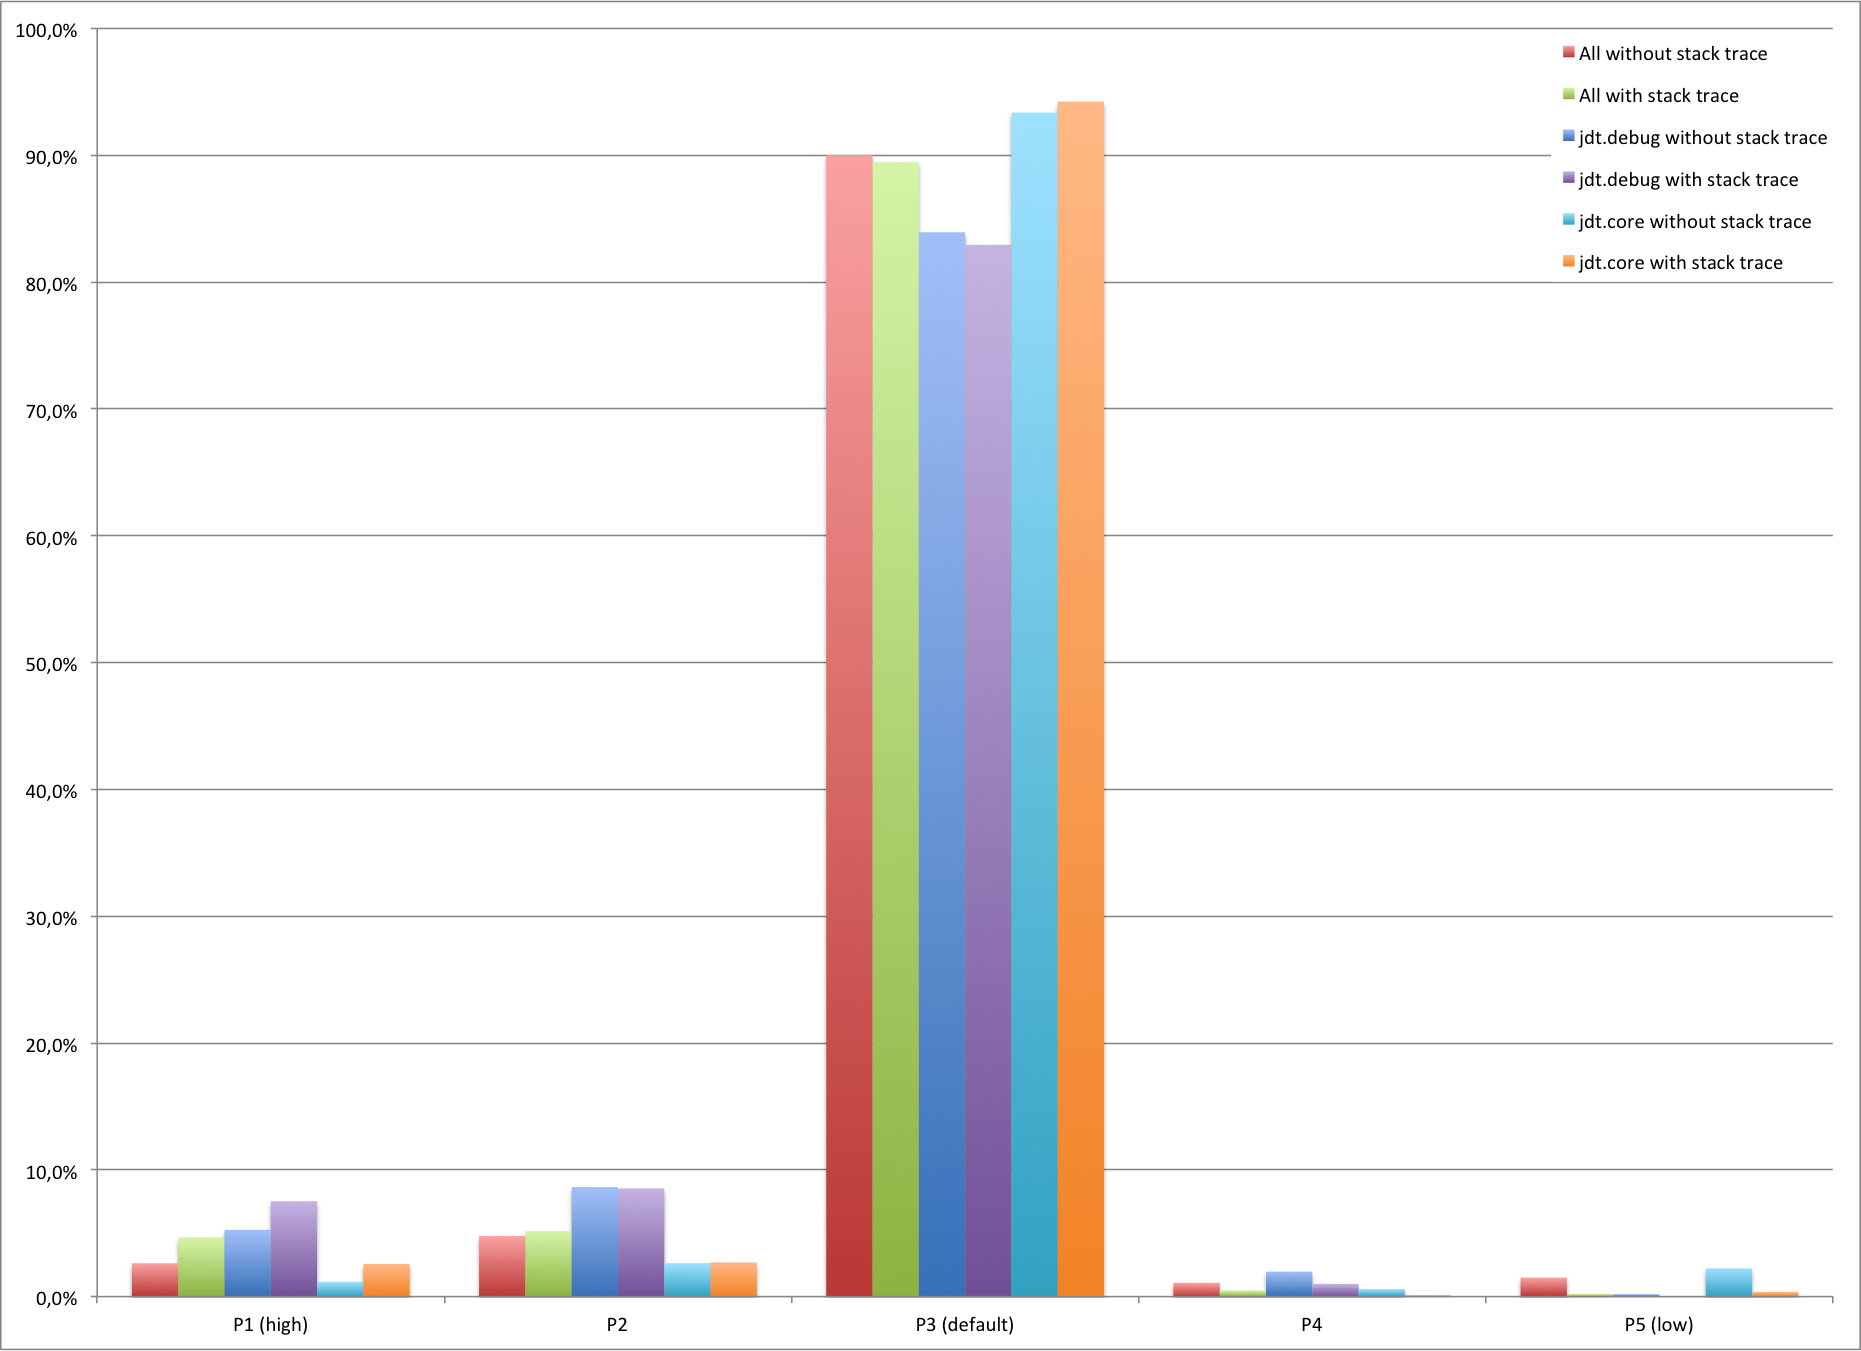
\includegraphics[width=1\textwidth]{img/priority.png}
	\caption{Distribution of priority for issues with and without stack traces.}
	\label{fig:priority}
\end{figure}
% subsection priority (end)

\section{Severity} % (fold)
\label{sec:severity}
Next to priority, every bug report is also assigned a severity. The severity of a bug report is expressed on a 7-level scale: 
\begin{inparaenum}[(1)]
\item blocker,
\item critical,
\item major,
\item normal,
\item minor, and
\item trivial. Also, a severity
\item enhancement is present.
\end{inparaenum}
The latter severity is discarded in this research, since it is used for enhancement requests, and not for bug reports.

Table~\ref{tab:severity} shows the distribution of the bug reports of the two projects, including a breakdown into bugs reports with and without a stack trace. The same data is also visualised in Figure~\ref{fig:severity}, showing a boxplot with and without outliers. Again, many outliers can be spotted in subfigure a.

Overall, 80\% of all bug reports have the default severity `normal'. Around one in ten bug reports is considered to have a major impact. Just like with the priority attribute, an overall shift towards the higher severity can be seen in the bar plot.  

When all bug reports are split into two groups, with and without stack traces, it seems that bug reports with a stack trace tend to have a higher severity. Whether or not there is a relation between the severity of a bug report and the presence of a stack trace is investigated in Section~\ref{sec:analysis_of_priority_and_severity_related_to_the_presence_of_a_stack_trace}.

\begin{table}[!ht]\footnotesize
	\centering
	\begin{tabular}{lrrrrrr}
		\toprule
		& jdt.debug && jdt.core && overall & \\
		\midrule
		All bug reports & 6,492 && 12,221 && 18,713 & \\
		\midrule
		Blocker & 70 & 1.1\% & 159 & 1.3\% & 229 & 1.2\%\\
		Critical & 267 & 4.1\% & 392 & 3.2\% & 659 & 3.5\%\\
		Major & 493 & 7.6\% & 1,170 & 9.6\% & 1,663 & 8.9\%\\
		Normal & 5,285 & 81.4\% & 9,781 & 80.0\% & 15,066 & 80.5\%\\
		Minor & 267 & 4.1\% & 579 & 4.7\% & 846 & 4.5\%\\
		Trivial & 110 & 1.7\% & 140 & 1.1\% & 250 & 1.3\%\\
		\\
		\midrule
		Bug reports without stack trace & 5,904 && 11,416 && 17,320 \\
		\midrule
		Blocker & 61 & 1.0\% & 136 & 1.2\% & 197 & 1.1\%\\
		Critical & 239 & 4.0\% & 352 & 3.1\% & 591 & 3.4\%\\
		Major & 433 & 7.3\% & 1,049 & 9.2\% & 1,482 & 8.6\%\\
		Normal & 4,809 & 81.5\% & 9,176 & 80.4\% & 13,985 & 80.7\%\\
		Minor & 256 & 4.3\% & 563 & 4.9\% & 819 & 4.7\%\\
		Trivial & 106 & 1.8\% & 140 & 1.2\% & 246 & 1.4\%\\
		\\
		\midrule
		Bug reports with stack trace & 587 && 805 && 1,392 \\
		\midrule
		Blocker & 9 & 1.5\% & 23 & 2.9\% & 32 & 2.3\%\\
		Critical & 28 & 4.8\% & 40 & 5.0\% & 68 & 4.9\%\\
		Major & 59 & 10.1\% & 121 & 15.0\% & 180 & 12.9\%\\
		Normal & 477 & 81.3\% & 604 & 75.0\% & 1,081 & 77.7\%\\
		Minor & 11 & 1.9\% & 17 & 2.1\% & 28 & 2.0\%\\
		Trivial & 3 & 0.5\% & 0 & 0.0\% & 3 & 0.2\%\\
		\bottomrule
	\end{tabular} 
	\caption{Statistics for severity.}
	\label{tab:severity}
\end{table}

\begin{figure}[!ht]
	\centering
		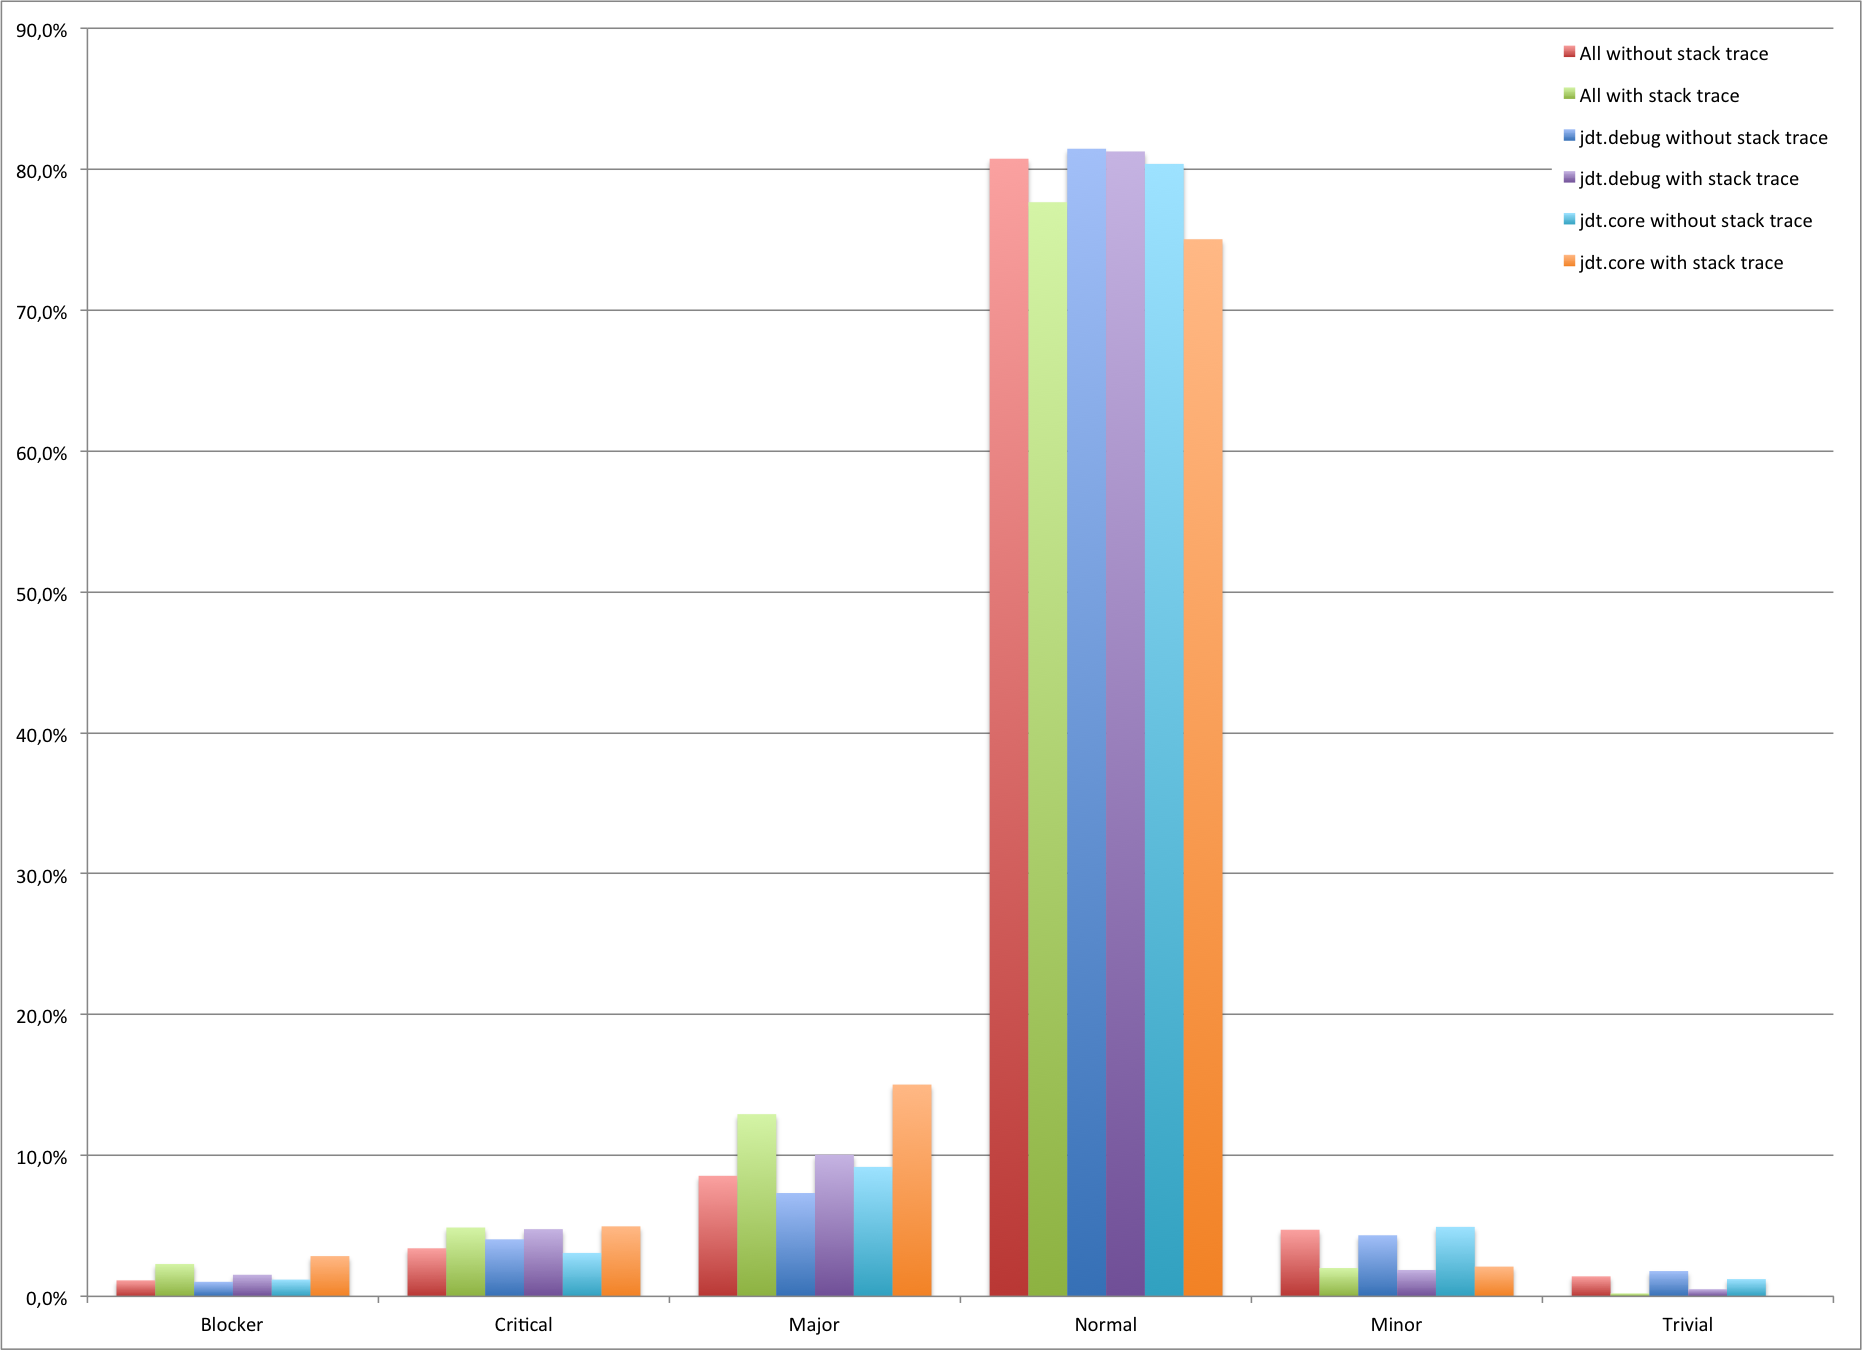
\includegraphics[width=1\textwidth]{img/severity.png}
	\caption{Distribution of severity for issues with and without stack traces}
	\label{fig:severity}
\end{figure}
% subsection severity (end)

\section{Time-to-fix} % (fold)
\label{sec:time_to_fix}
Figure~\ref{fig:ttf-stats} shows the time-to-fix distribution for bug reports for \texttt{jdt.debug}. Since only bugs that meet a specific search query are imported for \texttt{jdt.core}, data for this project is not shown. Some statistics are shown in Table~\ref{tab:ttf-stats}. For jdt.debug, around 30\% of all fixed bug reports have been fixed within a day. In this research, these bugs are discarded, since they probably are only created for administrative reasons. As can be seen, at least one bug is still open after over 8.5 years. The mean fix time is around three months, with a median fix time of 2.5 weeks. 

\begin{table}[!ht]\footnotesize
	\centering
	\begin{tabular}{lrrrrrr}
		\toprule
		project & min & max & mean & median & std \\
		\midrule
		jdt.debug & 1 & 3,137 & 95 & 18 & 225 \\
		\bottomrule
	\end{tabular} 
	\caption{Time-to-fix statistics for jdt.debug (in days).}
	\label{tab:ttf-stats}
\end{table}

\begin{figure}
        \begin{subfigure}[b]{0.48\textwidth}
                \centering
                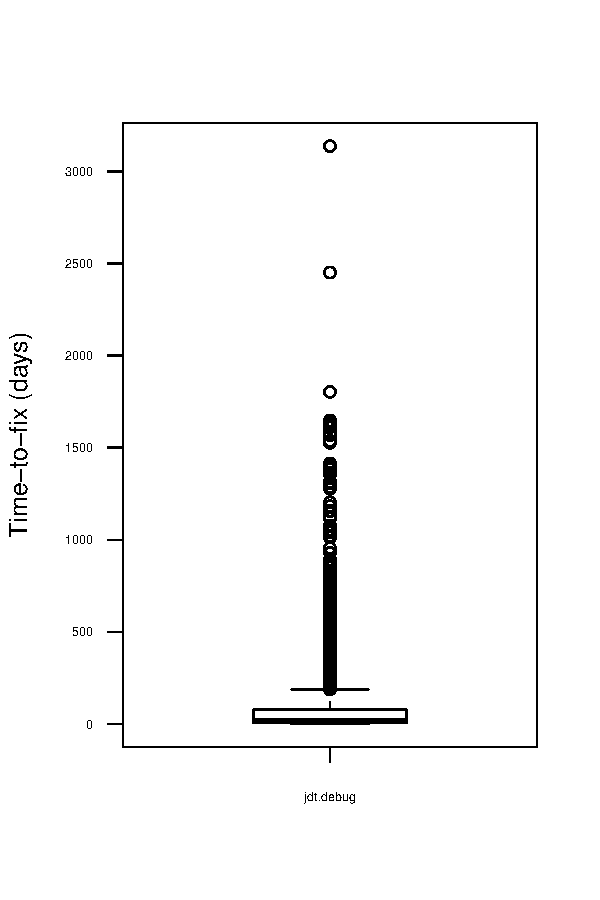
\includegraphics[width=\textwidth]{img/ttf.pdf}
                \caption{Time-to-fix (in days)}
        \end{subfigure}%
        ~ %add desired spacing between images, e. g. ~, \quad, \qquad etc. 
          %(or a blank line to force the subfigure onto a new line)
        \begin{subfigure}[b]{0.48\textwidth}
                \centering
                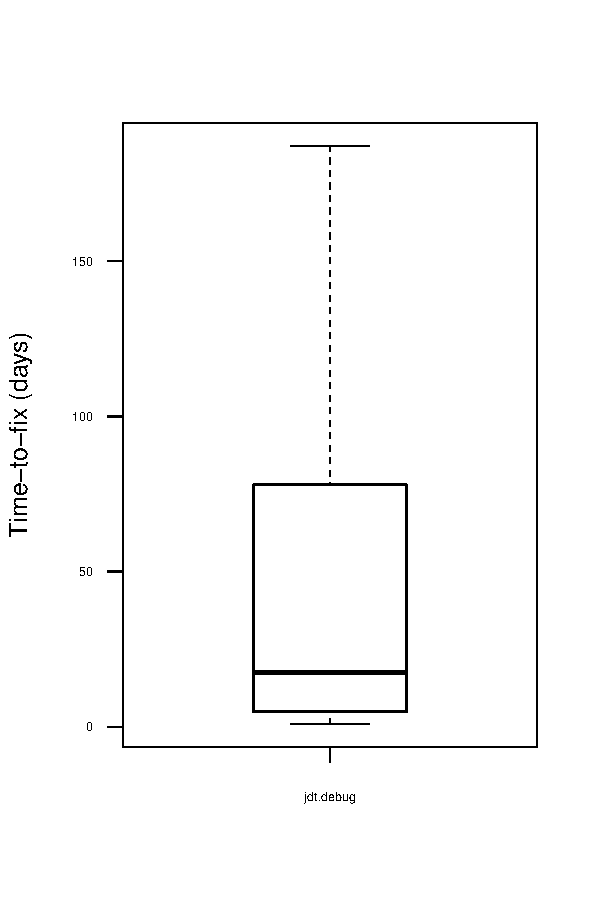
\includegraphics[width=\textwidth]{img/ttf-zoomed.pdf}
                \caption{Time-to-fix (without outliers, in days)}
        \end{subfigure}
		\caption{Time-to-fix statistics for jdt.debug}
		\label{fig:ttf-stats}
\end{figure}

% subsection time_to_fix (end)

\section{Class size} % (fold)
\label{sec:class_size}
Table~\ref{tab:class-stats} shows descriptive statistics for class size. For these measurements, the complete file history of each project is taken into account. For each class, the latest revision of that file is used for the lines of code measurement. The class size is also visualised in Figure~\ref{fig:class-stats}. Project's \texttt{jdt.debug} history contained 714 classes, \texttt{jdt.core} contained 1,715 classes. Please note these numbers include \emph{all} classes from the project history, also classes that are not present anymore in the latest revision of the project.

\begin{table}[!ht]\footnotesize
	\centering
	\begin{tabular}{lrrrrrr}
		\toprule
		project & N & min & max & mean & median & std \\
		\midrule
		jdt.debug & 714 & 2 & 2,628 & 73 & 15 & 198 \\
		jdt.core & 1,715 & 1 & 10,928 & 201 & 58 & 581 \\
		\bottomrule
	\end{tabular} 
	\caption{Class size statistics for each project (full history). N is the number of classes.}
	\label{tab:class-stats}
\end{table}
 
\begin{figure}
        \begin{subfigure}[b]{0.48\textwidth}
                \centering
                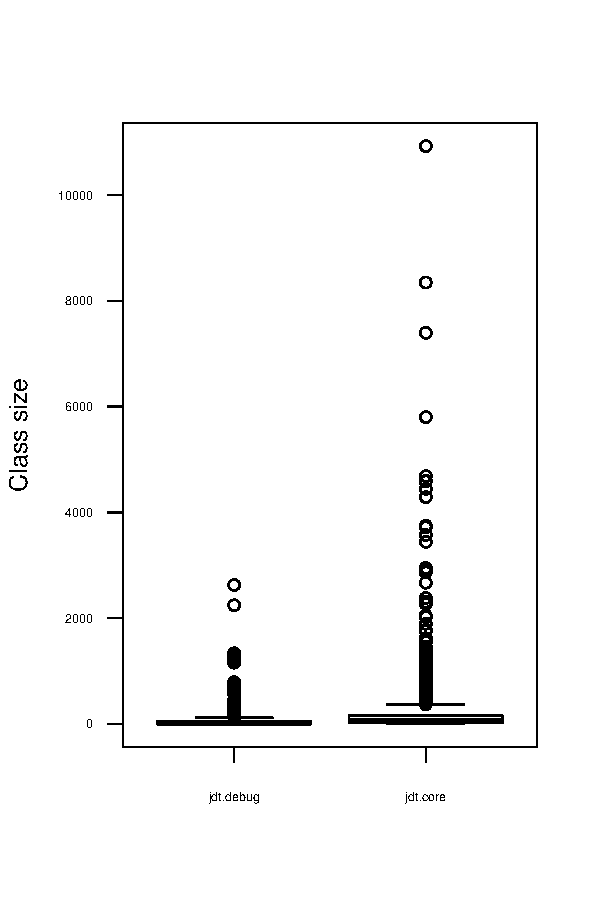
\includegraphics[width=\textwidth]{img/class-size-boxplot.pdf}
                \caption{Class size}
        \end{subfigure}%
        ~ %add desired spacing between images, e. g. ~, \quad, \qquad etc. 
          %(or a blank line to force the subfigure onto a new line)
        \begin{subfigure}[b]{0.48\textwidth}
                \centering
                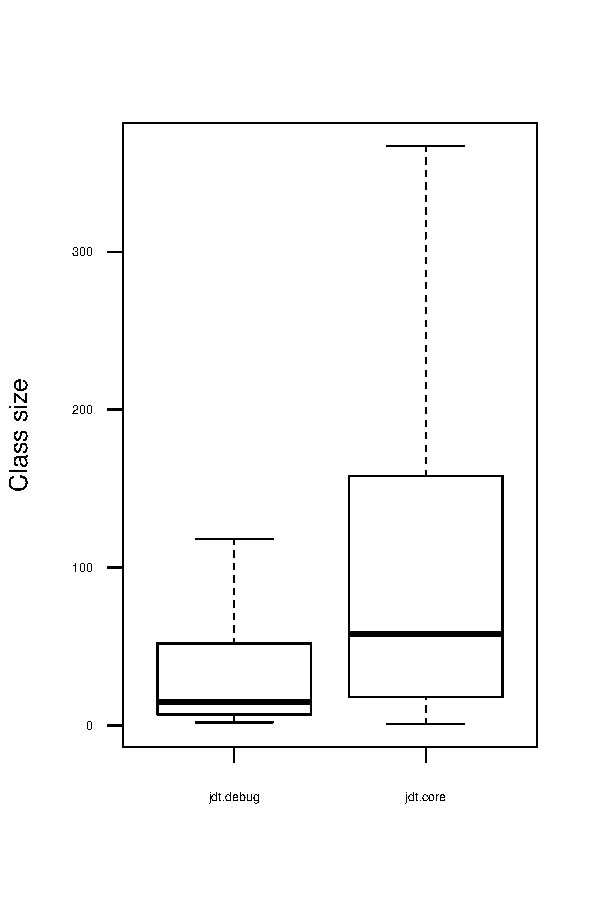
\includegraphics[width=\textwidth]{img/class-size-boxplot-zoomed.pdf}
                \caption{Class size (without outliers)}
        \end{subfigure}
		\caption{Class size statistics for each project (full history)}
		\label{fig:class-stats}
\end{figure}

When looking at the maximum number of lines of code, it can be seen that some classes have a very high number of lines of code. Although this looks quite odd, several source files in \texttt{jdt.debug} and \texttt{jdt.core} do indeed have such a high amount of lines of code ($> 30,000$, comments and white lines included\footnote{In Table~\ref{tab:class-stats}, white lines and comments are excluded, resulting in a far lower number.}). Also, there is quite a difference in mean (4.5 months) and median (almost 1.5 month) time-to-fix between \texttt{jdt.debug} and \texttt{jdt.core}. The box plot also shows this difference, where in subfigure b, the median value shows a particular shift, and the box plot for \texttt{jdt.core} spans a bigger range.
% subsection class_size (end)

\section{Package size} % (fold)
\label{sec:descr:package_size}
Table~\ref{tab:package-stats} shows the descriptive statistics for the three definitions of package size (see Section~\ref{sub:da:analysis_of_priority_and_severity_related_to_package_size}):

\begin{enumerate*}
	\item number of classes (NOC)
	\item total lines of code of associated classes (SUMLOC)
	\item (arithmetic) mean of lines of code of associated classes (AVGLOC)
\end{enumerate*}

The visualisations of these six measurements using a box plot are shown in Figures \ref{fig:package-stats} and \ref{fig:package-stats-zoomed}, where outliers are discarded from the latter box plot. For each underlying class, the latest revision is used for the lines of code measurement. Project \texttt{jdt.debug} contained 29 packages, \texttt{jdt.core} contained 65 packages. Please note these numbers include \emph{all} packages and classes from the project history, also packages and classes that are not present anymore in the latest revision of the project.

\begin{table}[!ht]\footnotesize
	\centering
	\begin{tabular}{lrrrrr}
		\toprule
		project & min & max & mean & median & std \\
		\midrule
		NOC\\
		\midrule
		jdt.debug & 4 & 178 & 49 & 32 & 47 \\
		jdt.core & 2 & 408 & 53 & 30 & 78 \\
		\midrule
		SUMLOC\\
		\midrule
		jdt.debug & 21 & 9,613 & 1,803 & 673 & 2,697 \\
		jdt.core & 2 & 36,798 & 5,313 & 2,099 & 8,024 \\
		\midrule
		AVGLOC\\
		\midrule
		jdt.debug & 1 & 129 & 37 & 18 & 40 \\
		jdt.core & 1 & 595 & 108 & 74 & 116 \\
		\bottomrule
	\end{tabular} 
	\caption{Package statistics for each project. Packages with no classes are discarded.}
	\label{tab:package-stats}
\end{table}
 
\begin{figure}
        \begin{subfigure}[b]{0.48\textwidth}
                \centering
                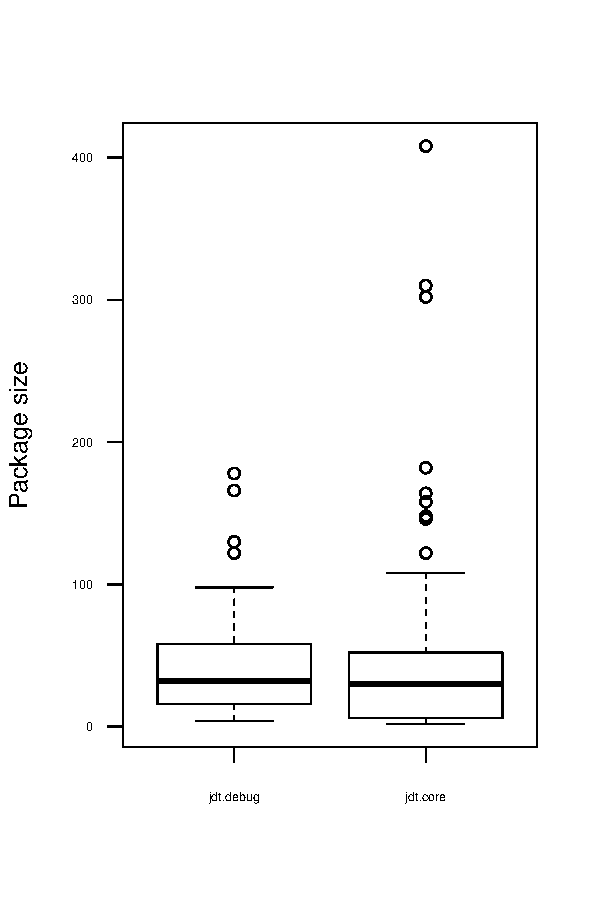
\includegraphics[width=\textwidth]{img/package-size-noc.pdf}
                \caption{NOC}
        \end{subfigure}%
        ~ %add desired spacing between images, e. g. ~, \quad, \qquad etc. 
          %(or a blank line to force the subfigure onto a new line)
        \begin{subfigure}[b]{0.48\textwidth}
                \centering
                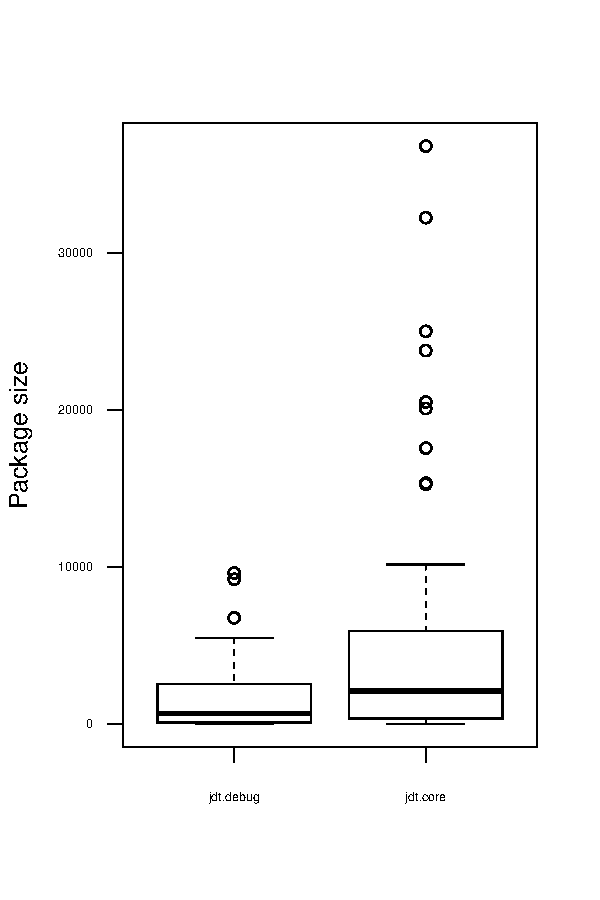
\includegraphics[width=\textwidth]{img/package-size-sumloc.pdf}
                \caption{SUMLOC}
        \end{subfigure}

        \begin{subfigure}[b]{0.48\textwidth}
                \centering
                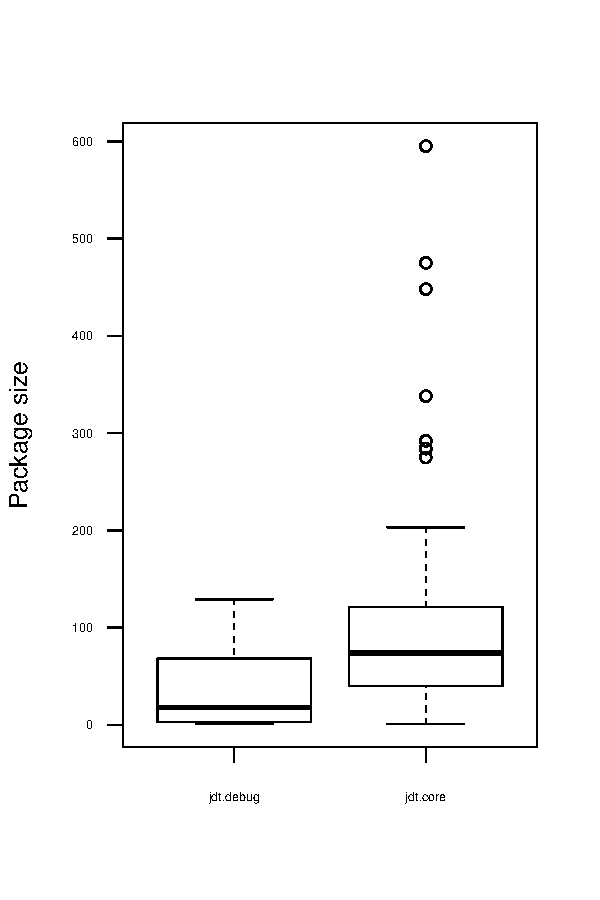
\includegraphics[width=\textwidth]{img/package-size-avgloc.pdf}
                \caption{AVGLOC}
        \end{subfigure}
		\caption{Package size statistics (full history). Packages with no classes are discarded.}
		\label{fig:package-stats}
\end{figure}

\begin{figure}
        \begin{subfigure}[b]{0.48\textwidth}
                \centering
                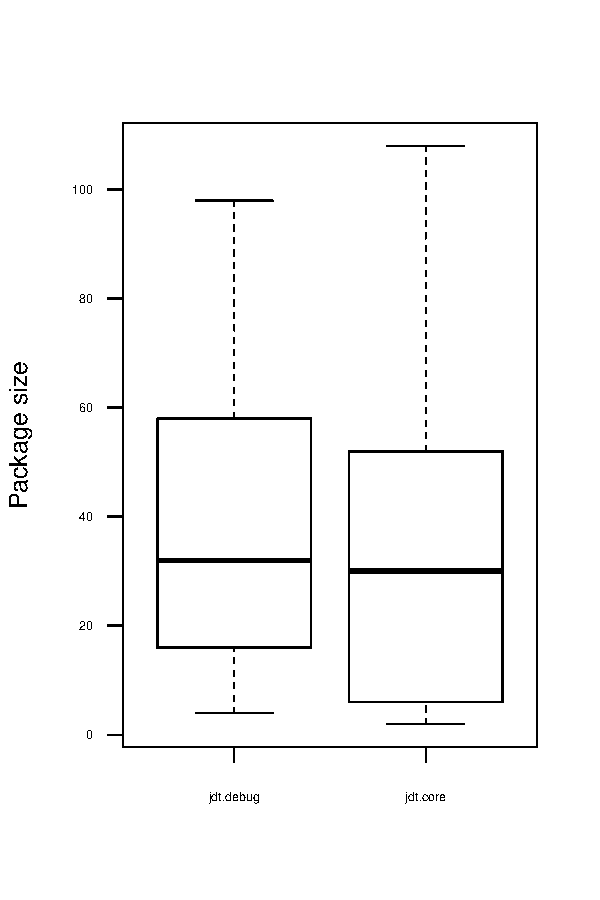
\includegraphics[width=\textwidth]{img/package-size-noc-zoomed.pdf}
                \caption{NOC}
        \end{subfigure}%
        ~ %add desired spacing between images, e. g. ~, \quad, \qquad etc. 
          %(or a blank line to force the subfigure onto a new line)
        \begin{subfigure}[b]{0.48\textwidth}
                \centering
                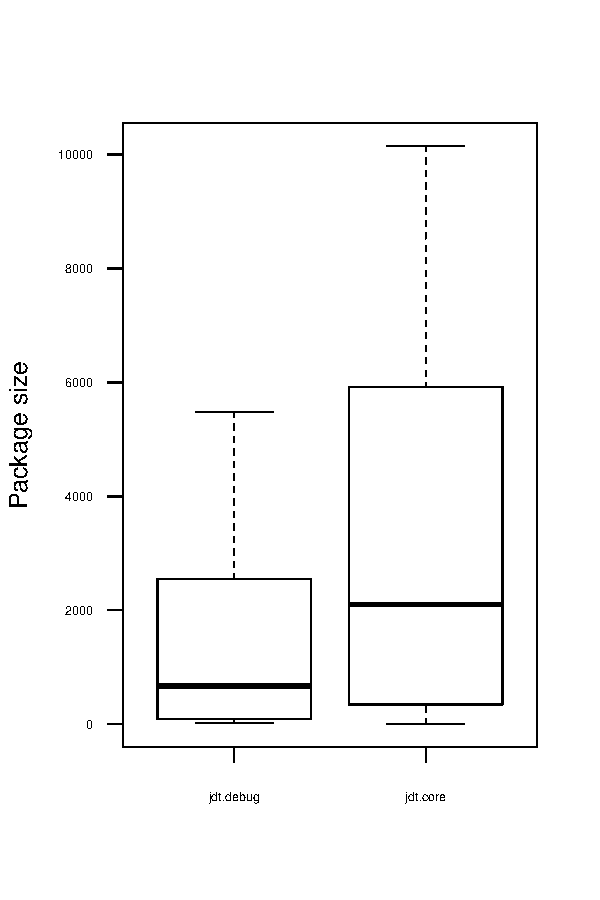
\includegraphics[width=\textwidth]{img/package-size-sumloc-zoomed.pdf}
                \caption{SUMLOC}
        \end{subfigure}

        \begin{subfigure}[b]{0.48\textwidth}
                \centering
                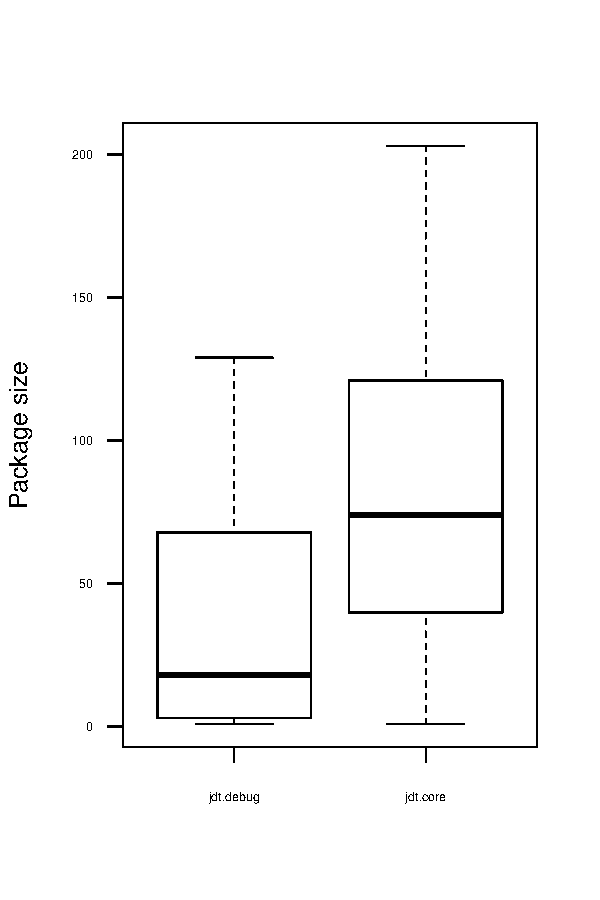
\includegraphics[width=\textwidth]{img/package-size-avgloc-zoomed.pdf}
                \caption{AVGLOC}
        \end{subfigure}
		\caption{Package size statistics (full history), without outliers. Packages with no classes are discarded.}
		\label{fig:package-stats-zoomed}
\end{figure}

A package in \texttt{jdt.debug} on average consists of 20 classes. This number increases to 26 for \texttt{jdt.core}. Some packages do not contain classes at all (they only contain sub-packages) and are discarded from the data set.

When looking at the total lines of code of the associated classes for a package (SUMLOC), it can be seen that some packages have a very high number of total lines of code. This is again due to the fact that several source files have a high amount of lines of code. The AVGLOC metric averages the total number of lines of all classes in a package over the number of classes in a package. This way, the influence of the number of classes in a package in cancelled out.

As can be seen in Figure~\ref{fig:package-stats-zoomed}, each package has a specific `signature' for each metric. This supports the theory that each software project should be treated in isolation, i.e., data sets should not be combined into one large data set.
% subsection package_size (end)

% chapter descriptive_statistics (end)